\section{The same model in a room}
\label{sec:room}

The room keeps the model family, the field head, the actor input, the cloning term, and both conditions, and removes everything else that makes the benchmark hard: there is one room, one station, no survival, and a successful episode can be four steps long.
Unlike on the benchmark, the station can be outside the image at the moment of the action itself (\cref{fig:room-crops}).

\begin{figure}[t]
  \centering
  \begin{subfigure}[t]{0.16\linewidth}
    \centering
    
\includegraphics[width=\linewidth]{room-crop-facing-station.png}
    \caption{Facing the station.}
  \end{subfigure}\hspace{1.5em}
  \begin{subfigure}[t]{0.16\linewidth}
    \centering
    
\includegraphics[width=\linewidth]{room-crop-facing-away.png}
    \caption{Facing away.}
  \end{subfigure}
  \caption{The $64\times64$ observation from the cell south of the station. Each tile is $16\times16$ pixels, one cell of the encoder's final feature map. (a) The station (orange) is in the nearest row. (b) The station is one cell behind the agent and absent from the image; \texttt{use} succeeds from here only in the behind-agent condition. These are environment frames, not reconstructions.}
  \label{fig:room-crops}
\end{figure}

\begin{table}[t]
  \centering
  \caption{The two conditions in the room, 8,000 environment steps each, one seed each. \emph{Teacher}: demonstrator episodes that scored. \emph{Actor \texttt{use}}: actor training episodes that scored, out of all actor episodes; \emph{last quarter} restricts this to the final quarter of training. \emph{Eval}: actor-only successes out of eight at about 2k, 4k, 6k, and 8k steps. \emph{Median length}: steps in a successful actor training episode; the demonstrator uses at step 52 (in crop) or 54 (behind agent).}
  \label{tab:room}
  \small
  % Generated by paper/scripts/build_assets.py. Do not edit.
\begin{tabular}{l l l r r l r}
\toprule
Station at \texttt{use} & Window & Teacher & Actor \texttt{use} & Last quarter & Eval (/8) & Median length \\
\midrule
in crop & anchored & 8/8 & 124/147 & 30/37 & 7, 7, 8, 8 & 36 \\
in crop & uniform & 8/8 & 85/110 & 25/28 & 5, 4, 6, 8 & 42 \\
behind agent & anchored & 8/8 & 185/190 & 48/48 & 8, 8, 8, 8 & 38 \\
behind agent & uniform & 8/8 & 130/138 & 35/35 & 7, 8, 8, 8 & 46 \\
\bottomrule
\end{tabular}

\end{table}

\begin{figure}[t]
  \centering
  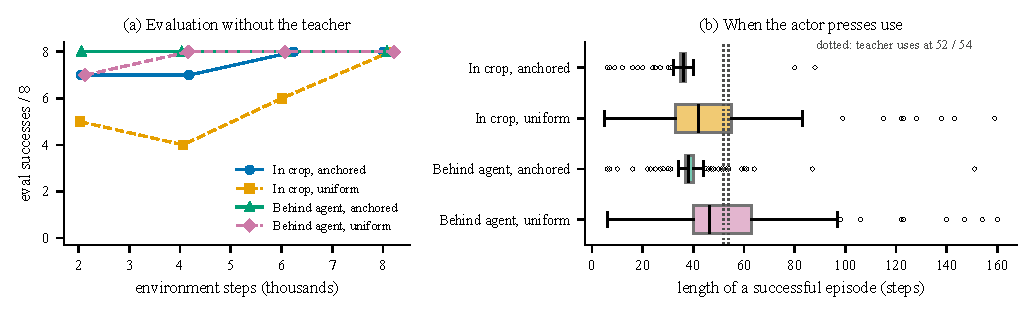
\includegraphics[width=\linewidth]{room_results.pdf}
  \caption{Room results, one seed per condition. (a) Actor-only evaluation successes out of eight. Solid lines are anchored windows, dashed lines uniform. (b) Length of every successful actor training episode. Dotted lines mark the demonstrator's \texttt{use} at step 52 (in crop) and 54 (behind agent).}
  \label{fig:room}
\end{figure}

\paragraph{The rare action is learned in every condition.}
\Cref{tab:room} and \cref{fig:room}(a) show that the actor learned \texttt{use} in all four runs.
Every run ended with eight of eight evaluation successes.
Every successful episode, in training and evaluation, was in the pose its condition requires, which the environment enforces.
Every failure was a 160-step timeout.
The behind-agent condition, in which the station is never in the image during the anchored window, was the more reliable of the two: \RoomOutAnchoredSuccess{} of \RoomOutAnchoredActor{} and \RoomOutUniformSuccess{} of \RoomOutUniformActor{} actor episodes scored, against \RoomInAnchoredSuccess{} of \RoomInAnchoredActor{} and \RoomInUniformSuccess{} of \RoomInUniformActor{} in crop, and its evaluations were at least seven of eight from the first one onward.
Removing the station from the image at the moment of the action did not prevent the action from being learned. That does not show the latent was supplying the station's location then. On real steps the field is the crop in front of the agent, so during the hold the station is in neither the image nor the field, and the facing-away probe's station cells are the four cells from the walk before the turn (\cref{tab:room-probe}). The latent does name the station on the frames where the station is visible (\cref{sec:latent}).

\paragraph{Anchoring changes when the actor acts, not whether.}
Uniform windows also learned the action in both poses.
What anchoring changed is the timing (\cref{fig:room}(b)).
With anchored windows, successful episodes cluster tightly: the median is \RoomInAnchoredMedian{} steps in crop and \RoomOutAnchoredMedian{} behind the agent, with 80\% of them between 31 and 38 steps and between 34 and 46 steps, respectively.
With uniform windows the medians are \RoomInUniformMedian{} and \RoomOutUniformMedian{}, and the middle 80\% spans 19 to 83 steps in crop and 28 to 84 behind the agent.
The in-crop uniform run was also the slowest to become reliable: its evaluations were 5, 4, and 6 of 8 before the final 8 of 8.
In every condition the actor acts well before the demonstrator's step 52 or 54, so it has not simply copied the length of the hold.

\paragraph{The room is not the benchmark.}
The room's \texttt{use} is one action from one cell in a fixed layout. The actor's first success came within the first 411 environment steps in every condition. Those steps count only the actor's interaction after training starts: the eight demonstrator episodes are collected before the loop and are not included.
The room shows that the recipe can produce the rare action in a layout where the station fills one encoder cell whenever it is in view, including a condition in which the station is behind the agent at the moment of acting. It does not show that the latent named the station during that hold.
It is not evidence that the recipe produces the benchmark's rare craft, which remained absent from every held-out life.
